%%%%%%%%%%%%%%%%%%%%%%%%%%%%%%%%%%%%%%%%%%%%%%%%%%%%%%%%%%%%%%%%%%%%%%%%
%
%
%     This file is included from the file   Segmentation.tex
% 
%     Section tag and label are placed in this top file.
%
%
%
%%%%%%%%%%%%%%%%%%%%%%%%%%%%%%%%%%%%%%%%%%%%%%%%%%%%%%%%%%%%%%%%%%%%%%%%



\piccaption[Zero Set Concept]{Concept of Zero Set in a Level Set.\label{fig:LevelSetZeroSet}}
\parpic(9cm,6cm)[r]{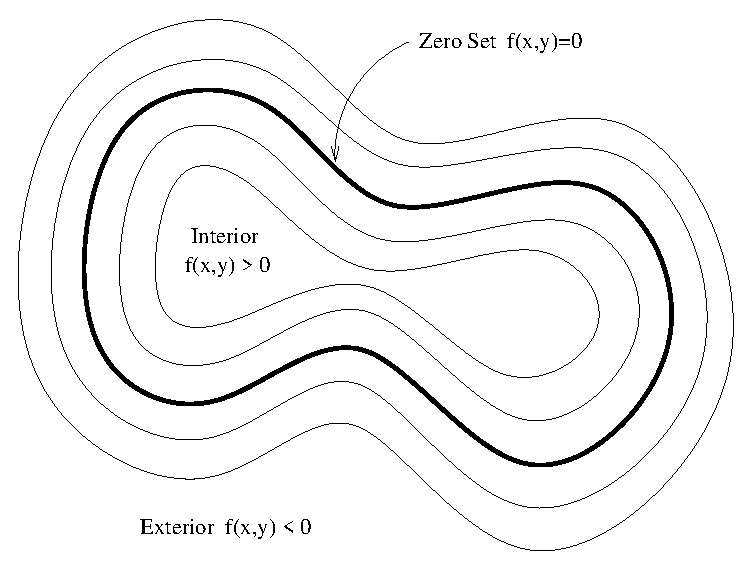
\includegraphics[width=8cm]{LevelSetZeroSet.eps}}

The paradigm of Level Set for performing image segmentation is based on
representing the boundary of an object by using the \emph{zero set} of a
function. Modifications applied to the function parameters will result in
displacements and shape changes of its zero set. It can be said that the object
boundary is defined as an implicit function of the form $f(\bf{X})=0$. 

In the typical approach to Level Set segmentation the contour is initialized by
the user and then is made evolve in order to make it fit to the form of an
anatomical structure in the image. The evolution of the \emph{zero set} is
simulated by changing the $f$ function under the control of a differential
equation.  The terms in the equation basically represent a diffusion equation
in which the speed term can be customized by the user.

Many different implementation and variants of this basic concept have been
published in the literature. A overview of the field has been made by Sethian
\cite{Sethian1996}. The following sections introduce practical examples of some
of the Level Set segmentation methods available in ITK.


\subsection{Fast Marching Segmentation}
\label{sec:FastMarchingImageFilter}

\ifitkFullVersion
\input{FastMarchingImageFilter.tex}
\fi



\subsection{Shape Detection Segmentation}
\label{sec:ShapeDetectionLevelSetFilter}

\ifitkFullVersion
\input{ShapeDetectionLevelSetFilter.tex}
\fi


\subsection{Geodesic Active Contours Segmentation}
\label{sec:GeodesicActiveContourImageFilter}

\ifitkFullVersion
\input{GeodesicActiveContourImageFilter.tex}
\fi



\subsection{Threshold Level Set Segmentation}

\subsection{Segmentation Level Set Image Filter}
\label{sec:SegmentationLevelSetImageFilter}


